Det här är teori\cite{einstein}. \\
Hänvisning till \cref{eq:namn}
\begin{equation} \label{eq:namn}
    E=m \cdot c^2.
\end{equation}

Hänvisning till \cref{tab:namn}.
\begin{table}[H]
\caption{Namn} \label{tab:namn}.
\centering 
    \begin{tabular}{|c|c|c|}
    \hline
    \textbf{Storhet} & \textbf{Symbol} & \textbf{Dimension} \\
     \hline
Energi &  $E$ & $ML^2T^{-2}$ \\
    \hline
Massa & $m$ & $M$ \\
    \hline
Ljusets hastighet & $c$ & $LT^{-1}$ \\
    \hline
    \end{tabular} 
\end{table}

Hänvisning till \cref{fig:namn}.
\begin{figure} [H]
    \centering 
    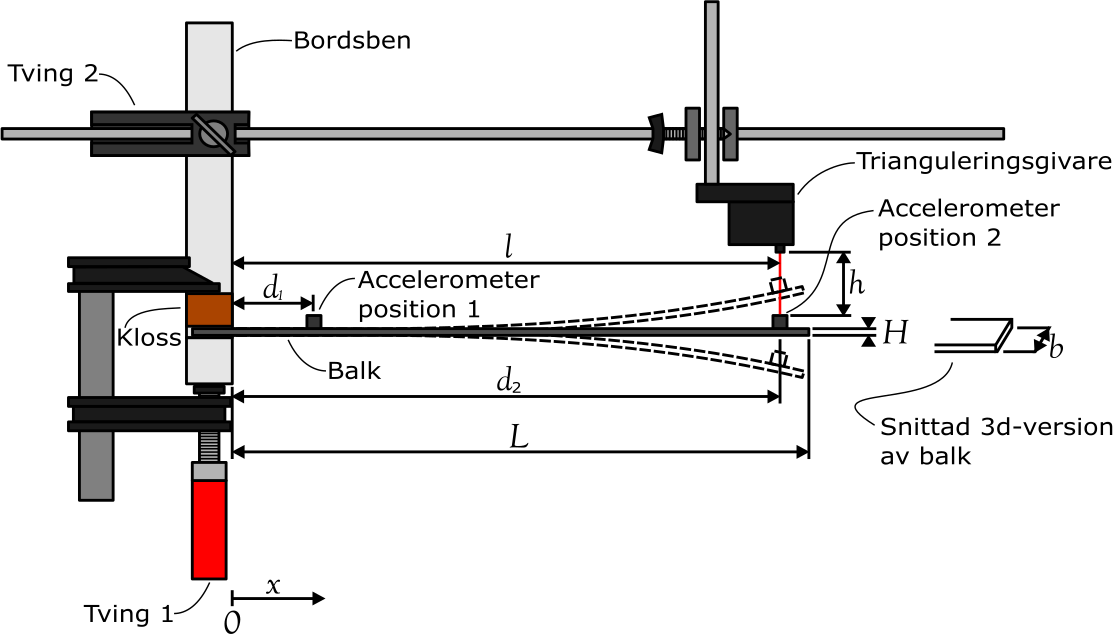
\includegraphics[width=0.5\textheight]{experiment_uppstallning.png}
    \caption{Beskrivande text.}
    \label{fig:namn}
\end{figure}